\section{What are some choices you made about how to raise your children?}
    1. John and I grew up without TV in our homes. 
Radio came to our house around the time I turned 9 years old. 
Interestingly it was the decision of the Lancaster Conference Bishop Board to relax their decree on "no radios" that freed my parent to purchase a turntable and radio console. 
I remember listening to two events by radio, funeral of President Kennedy and wedding of Luci Johnson.  
I'm not sure if the radio was borrowed or if my parents had already purchased their radio. 
I say all of that to say that after there was a radio in the house we listened to certain radio programs like clockwork. 
It was every afternoon at 4 or 4:30 that we listened to Ranger Bill or Aunt Bertha. 
This habit had an impact in my way of thinking. 

When it came to teaching and training my children I was concerned about the impact of allowing an influence from secular society to regularly impact the thinking of young minds. 
I wanted my children to think for themselves and have an inquiring skepticism of popular culture. 
So we limited the amount of time you watched TV as well as the content.

    2. I breast fed my babies and felt that provided a healthy nutritional start for your lives. 
It also seemed the natural and normal action. 
Interestingly my mother choose to not breast feed me, at least not for very long. 
Here is the recipe for the formula I must have drunk. 
Notice that the date is March 1953 this could mean that my Mom did breast feed me for a few months. 
She is not here to ask and I can't remember. 
I was quite surprised to see the amount of sugar included in each batch of 5 eight ounce bottles. 
Is it a wonder that I have a sweet tooth?

\begin{figure}
\centering
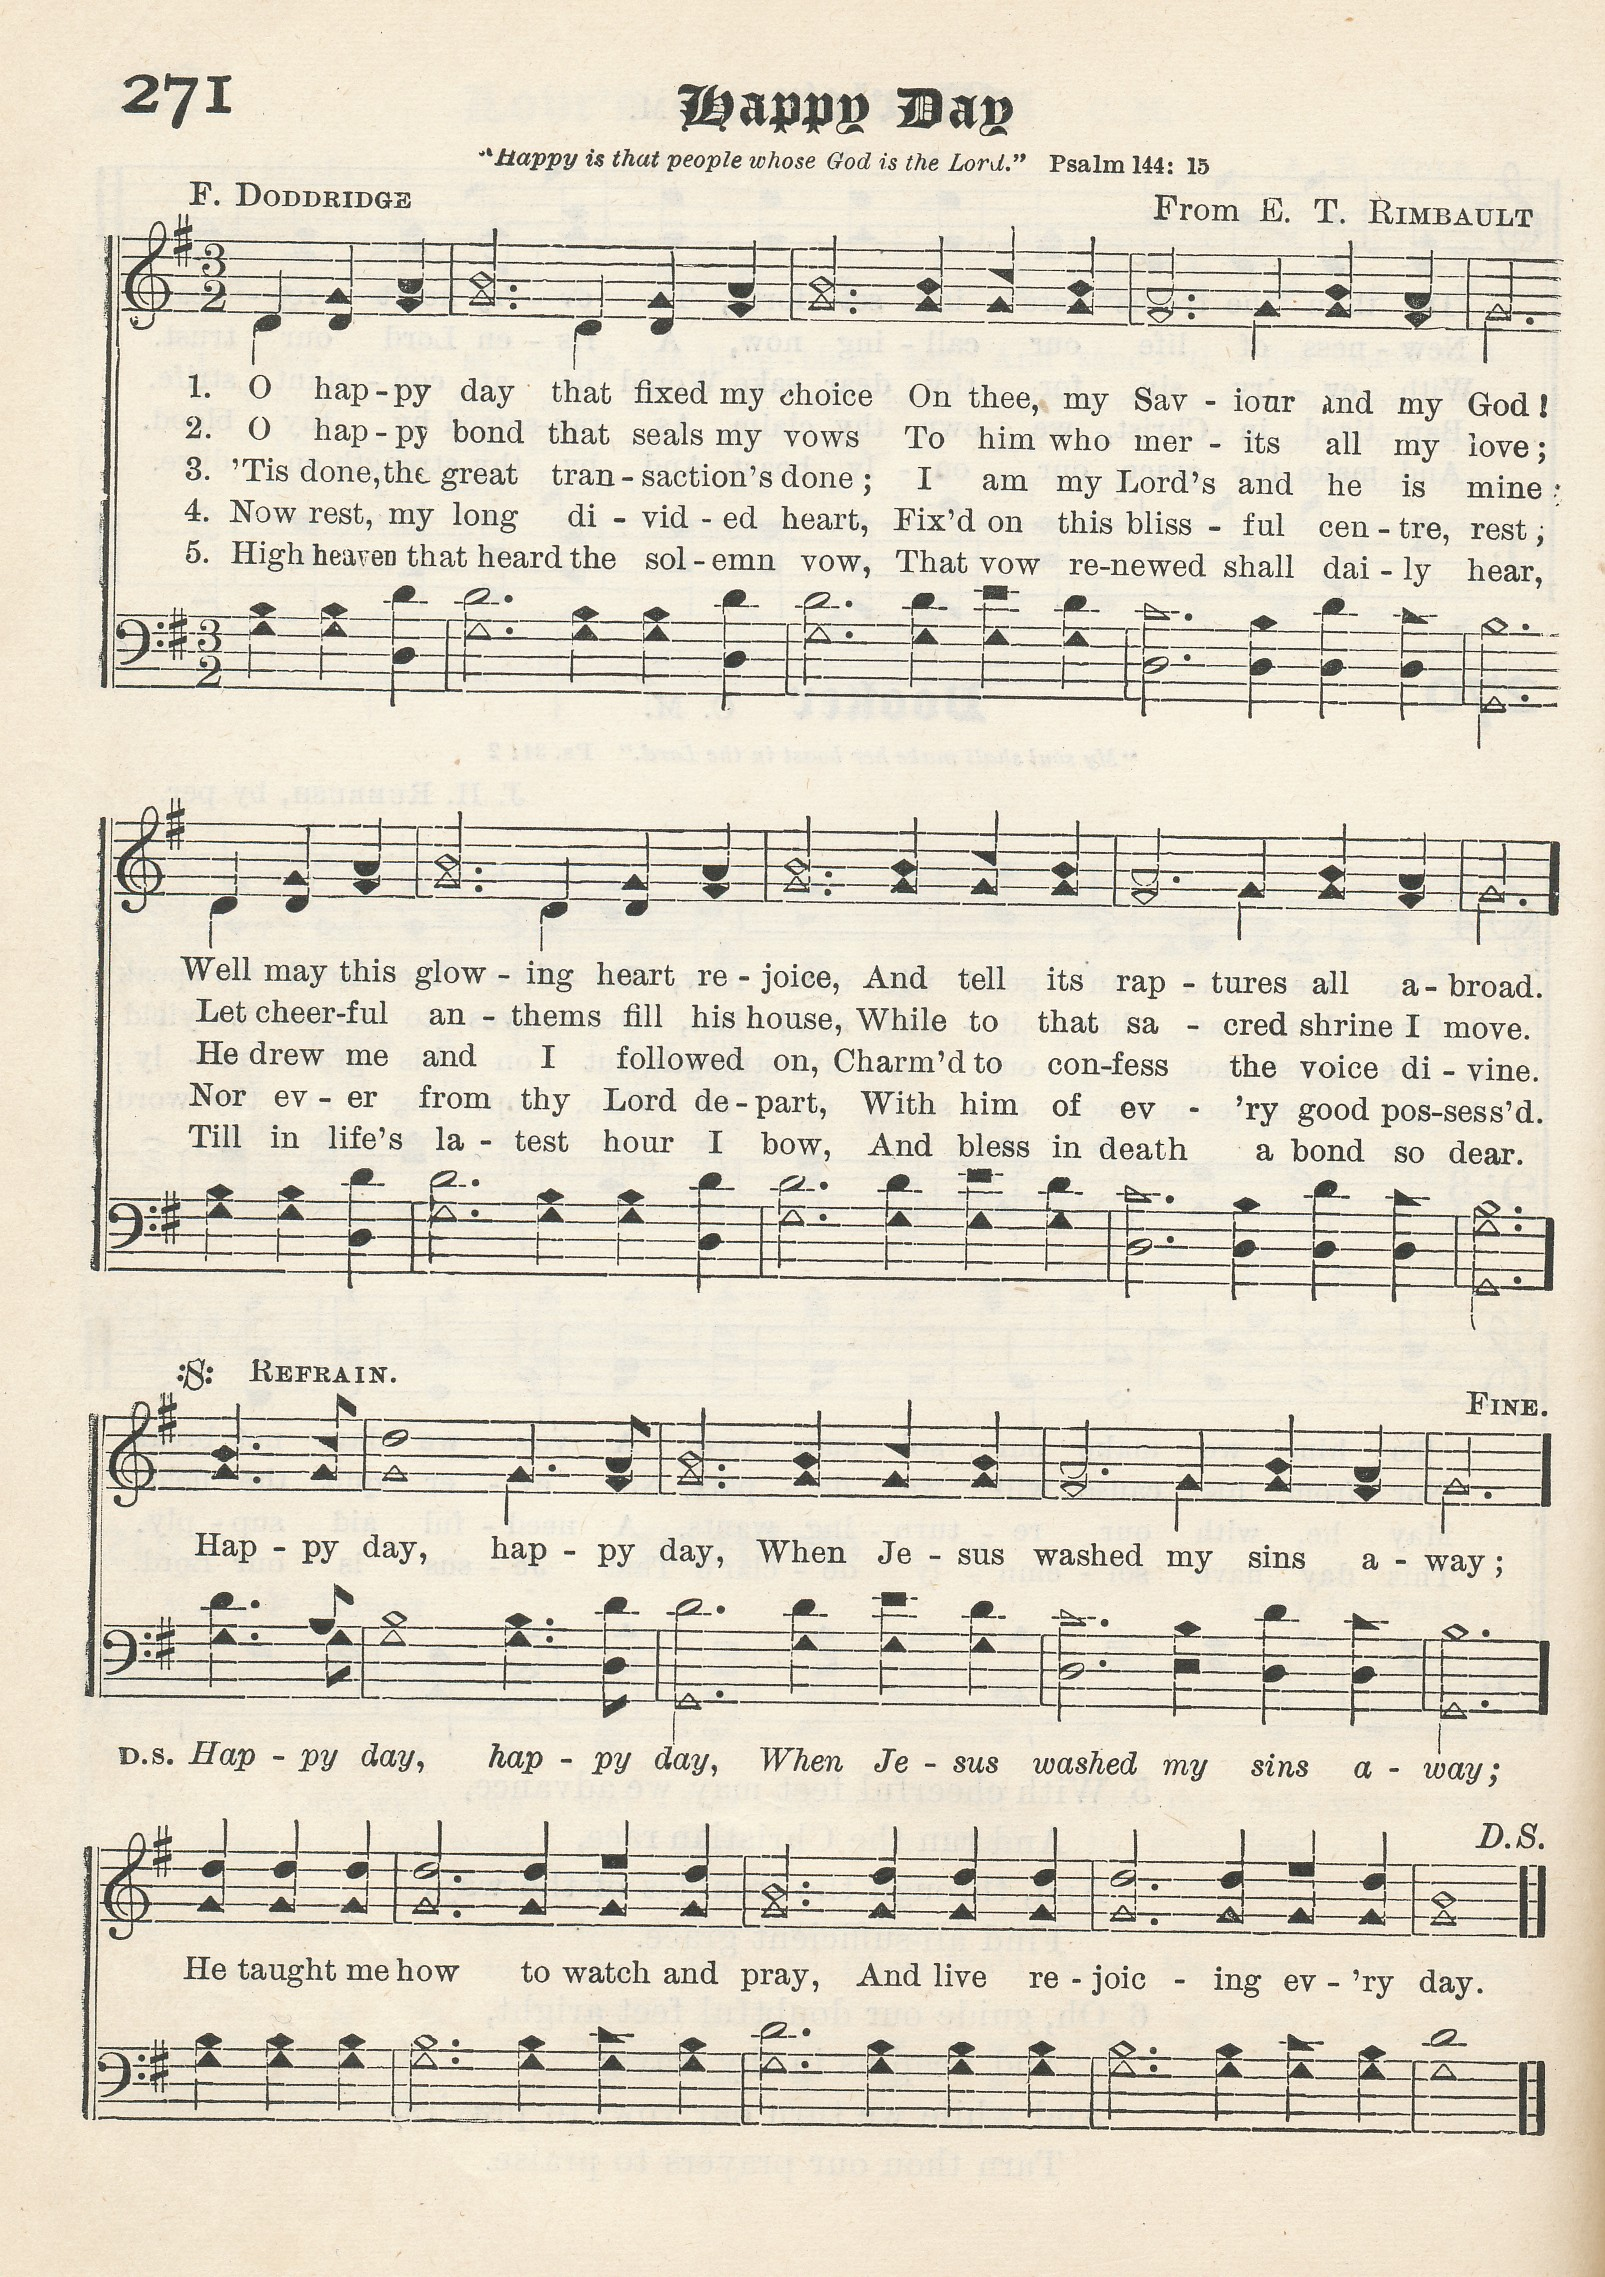
\includegraphics[width=0.9\textwidth]{our_family/19.jpg}
\caption{
Recipe for formula
}
\end{figure}

    3. We chose to invest in Tyco/Lego building blocks and I enjoyed the hours you all spent creatively building and playing with them.





